\documentclass[10pt,final,journal]{IEEEtran}
\usepackage[english]{babel}
\usepackage{listings}
\usepackage{graphicx}
\usepackage{caption}
\usepackage{subcaption}
\usepackage{amsmath}
\usepackage{color}
\usepackage{cite}
\usepackage{url}
\usepackage{algorithm}
\usepackage{algpseudocode}

\graphicspath{{./images/}}

\usepackage[margin=1in]{geometry}

\definecolor{mygray}{rgb}{0.4,0.4,0.4}
\definecolor{mygreen}{rgb}{0,0.8,0.6}
\definecolor{myorange}{rgb}{1.0,0.4,0}

\definecolor{lightgray}{rgb}{.9,.9,.9}
\definecolor{darkgray}{rgb}{.4,.4,.4}
\definecolor{purple}{rgb}{0.65, 0.12, 0.82}

\DeclareMathSizes{10}{10}{10}{10}

\lstset{
backgroundcolor=\color{lightgray},
extendedchars=true,
basicstyle=\footnotesize\ttfamily,
showstringspaces=false,
showspaces=false,
numbers=left,
numberstyle=\footnotesize,
numbersep=9pt,
tabsize=2,
breaklines=true,
showtabs=false,
captionpos=b
keywordstyle=\color{blue}\bfseries,
ndkeywordstyle=\color{darkgray}\bfseries,
identifierstyle=\color{black},
commentstyle=\color{purple}\ttfamily,
stringstyle=\color{red}\ttfamily,
}

\title{Embedded Lab Assignment 2\\\small{Group 7}}
\author{
		\IEEEauthorblockN{
			Haji~Akhundov\IEEEauthorrefmark{1}
			Misael~Hernandez~Leal\IEEEauthorrefmark{2}
			Fei~Tan\IEEEauthorrefmark{3}
			Koray~Yanik\IEEEauthorrefmark{4}
			Muneeb~Yousaf\IEEEauthorrefmark{5}
		}

		\IEEEauthorblockA{
			\IEEEauthorrefmark{1}h.akhundov@student.tudelft.nl			\small{4390547} \and
			\IEEEauthorrefmark{2}m.a.hernandezleal@student.tudelft.nl 	\small{4423615} \and 	\\
			\IEEEauthorrefmark{3}f.tan@student.tudelft.nl 				\small{4405722} \and
			\IEEEauthorrefmark{4}k.i.m.yanik@student.tudelft.nl 		\small{4382781} \and 	\\
			\IEEEauthorrefmark{5}m.m.yousaf@student.tudelft.nl 			\small{4411129}
		}
}

\date{\today}

\begin{document}

\nocite{*}

\maketitle

\begin{abstract}
This report describes the optimization process of an existing sequential image processing algorithm, namely edge detection on a heterogeneous system with multiple processing units.

Given the reference application, we rewrite the code such that it runs on an embedded system, utilizing a digital signal processor (DSP) and parallel computation extensions (SIMD) (TI Processor, NEON) to achieve a speedup over a purely sequential reference implementation.
\iffalse The application was implemented on a TI processor that includes an ARM core with NEON support and a DSP.\fi
Profiling the reference application shows that 80\% of the effort (or time?) is spent on the gaussian filtering function. Further investigation showed that the function could distribute its workload to available processing units. By carefully load balancing this function
 \iffalse between the two available processing units mentioned, \fi
 we were able to achieve an approximate speedup of a factor of two.
We describe
the difficulties of working with this system, go into some depth about the 
obtained speedup and discuss further improvements that could be made.

\end{abstract}

\newpage

\section{Introduction}
\textbf{A lot of this can still be reused,  We should also mention "hardware software co-design" somewhere here}
The purpose of this assignment is to improve a sequential version of an image processing algorithm on a multi-core heterogeneous computing platform provided. The given platform is the Beagle Board\footnote{http://beagleboard.org/} that has a general purpose ARM processor (from now on referred to as the \emph{GPP}) and a digital signal processor (\emph{DSP}) that would be utilized in this lab for the edge detection algorithm and eventually obtaining a speed up by performing computations in parallel. Luckily the heavily used gaussian filtering function \textbf{(see Section 2. Profiling) change this to an actual link} could be load balanced among different processing units due to its very little data dependency. \textbf{bla bla bla..... }

\subsection{Overview}
Figure~\ref{fig:workflow} shows the reader the overall approach to this problem and the basic work flow that we adhered to. In this report we will go through describing each component in the flow diagram presented. We would also discuss the communication model that was used to communicate the necessary data in the heterogeneous environment, and see that the communication model (ie. shared memory) used here has little overhead and imposes almost no additional delays when compared to the communication model(ie. message passing) that was utilized in the previous lab. The application profiling has made a great impact on steering our decisions as we will see (in Section Profiling). Furthermore every core has a hardware limitation in terms of how many operations can be performed at the same time, which defines the upper bound on how much speed-up can be obtained. At last results and their error verification are presented. In the future improvements sections we discuss what are the potential possibilities to further improve the execution speed of the application.

\begin{figure*}
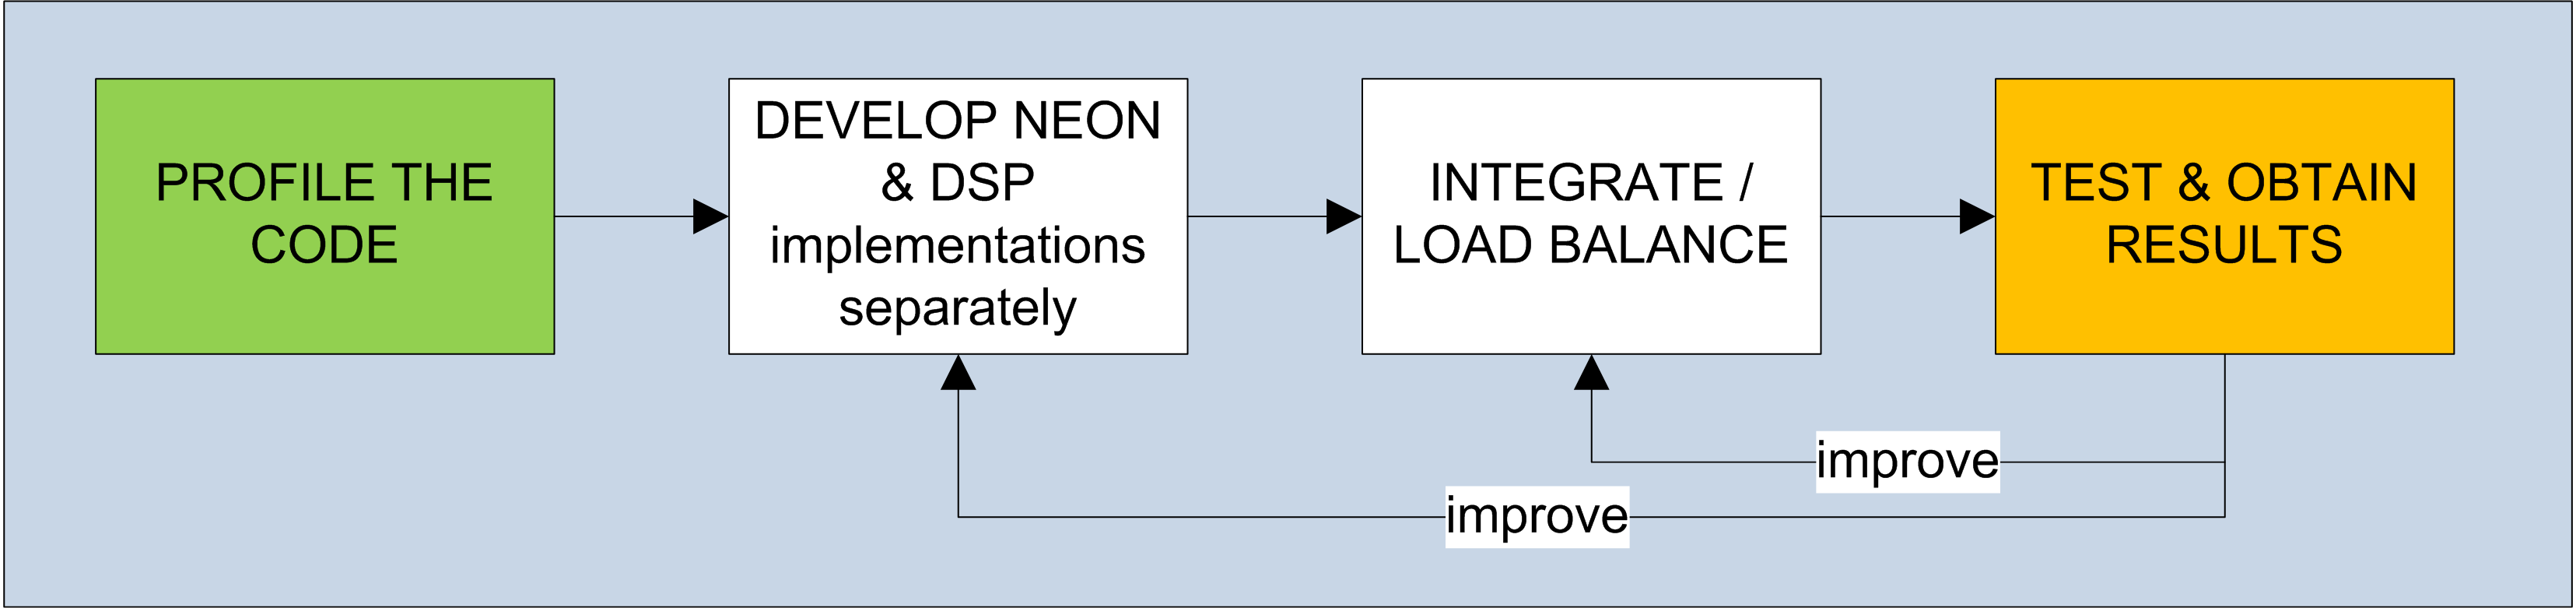
\includegraphics[width=\linewidth]{drawings/workflow}
\caption{General approach to the problem}
\label{fig:workflow}
\end{figure*}




\section{Profiling}

The space and timing complexity of the any application is measured by the profiling. In this assignment, MCProf profiling tool is being used for the profiling of the  \emph{Canny Edge Detection} application. MCProf is a  runtime Memory and Communication profiler which generates detailed application profile in terms of memory access patterns and data-communication at function and loop-level granularity. we did  profiling  of this application for the given sample pictures and realized that gaussian-smooth function consumes almost 80\% of the processing time for each input picture. Moreover,for each picture most of the memory accesses is also done from this function. Therefore, we decided to accelerate this function. The profiling results for the \emph{tiger.pgm} input image is shown in the  following diagrams. 

The profiling results of the rest of the pictures are attached in the appendix

\section{Implementation}

\begin{figure}
\centering
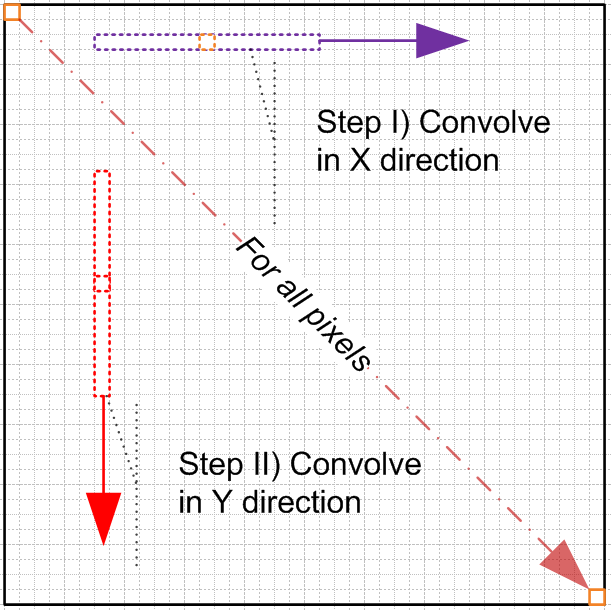
\includegraphics[width=0.4\textwidth]{drawings/gaussian_general}
\caption{Convolution process}
\label{fig:convolution}
\end{figure}

Obtaining the results from profiling we see that approximately 80\% of the time is spent on executing the \textit{gaussian\_smooth} function. Observing the code of this function we see that it is divided into two for loops (also seen in profiling output in figure~\ref{fig:prof}).
First the blurring is done by convolution in the X-direction and then in the Y-direction by applying the gaussian kernel (one dimensional convolution matrix). This process is briefly shown in figure~\ref{fig:convolution}. There is a data dependency between the two convolution processes where one must be followed by the other, so simply performing one convolution in one direction on one processing unit and the other direction on a different processor will not work.


\begin{figure}
\centering
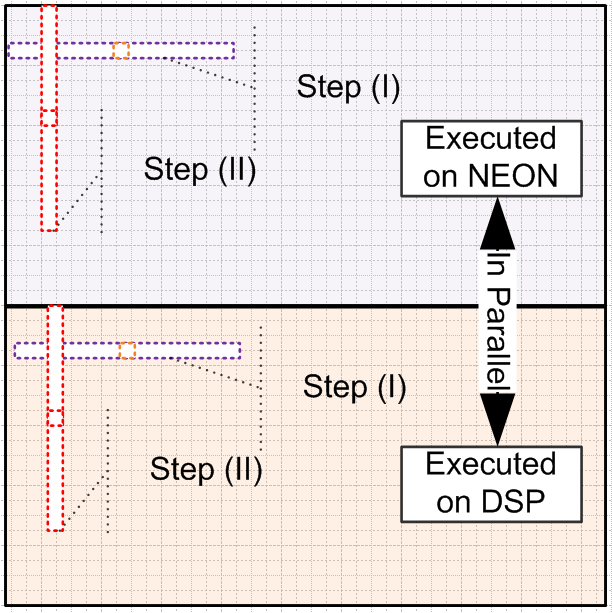
\includegraphics[width=0.4\textwidth]{drawings/gaussian_balancing}
\caption{Splitting the work}
\label{fig:balancing}
\end{figure}


The most naive way of splitting the work between two processors and obtaining a speed-up is to compute the gaussian filtering on both processors for different parts of the image. The most simplistic way with a 50/50 load balancing is depicted in figure~\ref{fig:balancing} where the NEON is performing the convolutions on the top part of the image and the DSP performs the convolutions on the bottom part of the image. As shown in the workflow diagram in figure~\ref{fig:workflow} we then proceed with the development of the gaussian filtering independently on each processor and later use clever techniques to split the computation between the two processors.


\begin{figure}
\centering
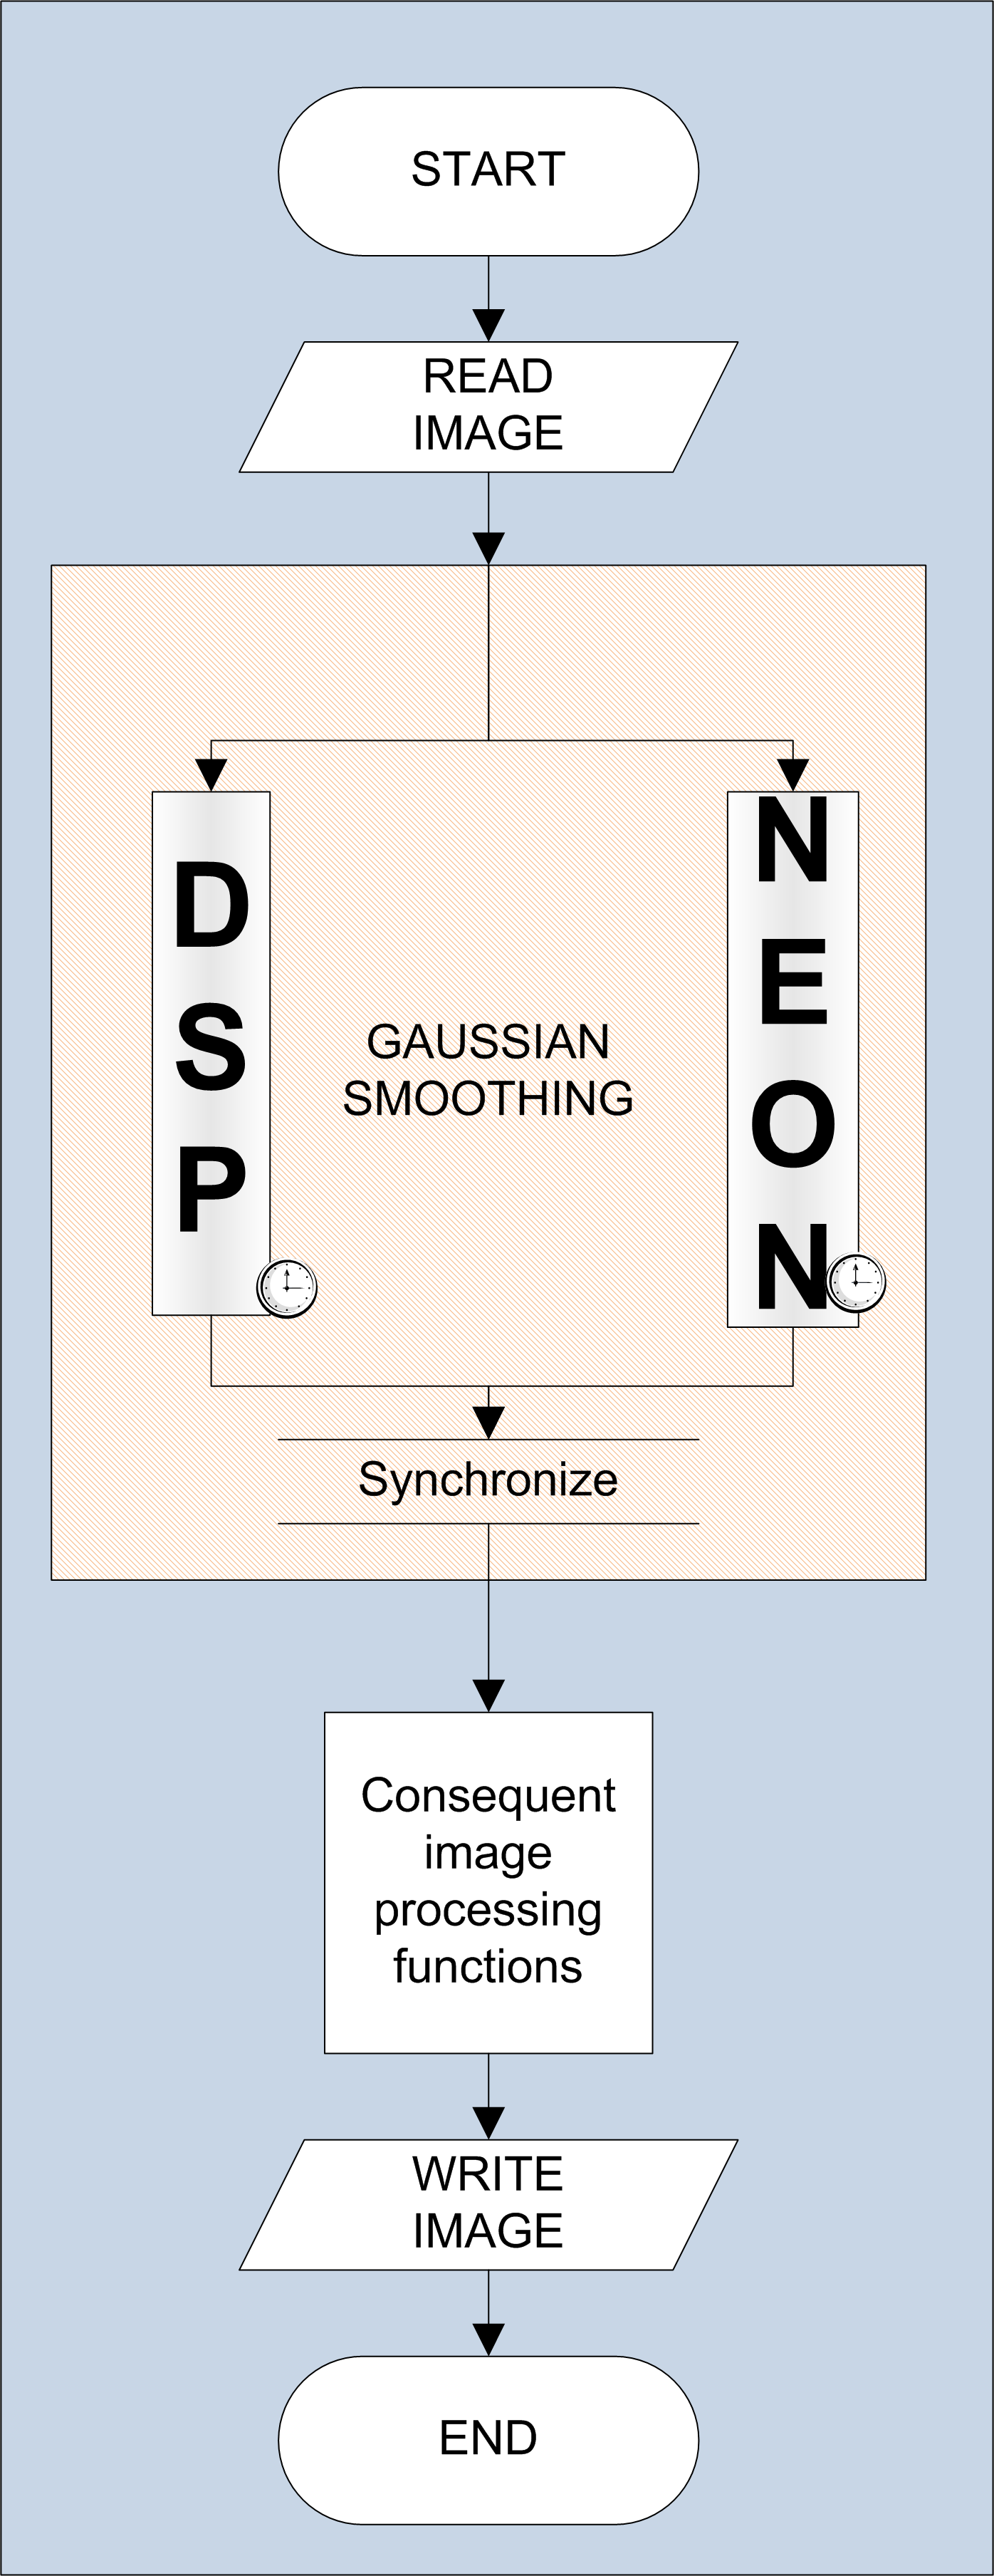
\includegraphics[width=0.25\textwidth]{drawings/model}
\caption{Data flow}
\label{fig:dataflow}
\end{figure}


On the GPP side we define FRAC which is an integer value from zero to hundred that specifies the fraction of calculations that must be done on the NEON. After integrating both compute units and making them work in parallel, both instances of gaussian smoothing calculations were measured in time and a FRAC that resulted in an even balance between GPP and DSP was chosen. Note that the two calculations have to be completed before the program can resume.
Hence, by load balancing we make sure that the synchronization happens as soon as possible and very little time is wasted on waiting for the slower processor to finish. Figure~\ref{fig:dataflow} shows the resulting dataflow of the current implementation. The subsequent sections go into more details of this process.


\section{DSP}
The \emph{OMAP3530} general purpose processor (from now on referred to as the
\emph{GPP}) contains a \emph{TMS320} digital signal processor (\emph{DSP}). This
core is optimised for using multiple calculation channels simultaneously: it is
a \emph{VLIW} (Very Long Instruction Word) processor that can utilise eight
functional units at the same time. More specifically, we can use six ALUs and
two multipliers per instruction. Another interesting feature is that each
multiplier can perform two 16 x 16-bit multiplications as well, giving us
potentially four multiplications in parallel.

The GPP unit is responsible for starting up the DSP core, giving it an executable to run
and afterwards detaching the core. Furthermore, the requirements specified
that the matrices to multiply are generated on the GPP core (which is 
of course not a bad idea because the GPP is way more flexible: it can easily
be changed to read the matrices from a file or standard input, and we can
offload a part of the work to the GPP itself and also the \emph{NEON} as we 
will discuss later as well). 

\subsection{Communication}
This however brings us to one complication: the matrices have to be moved to
the DSP core, while the (partial) end result has to be sent back to the GPP.
Our first goal is thus to set up communications and send matrices back and forth
between the two cores. 

\begin{figure}[h]
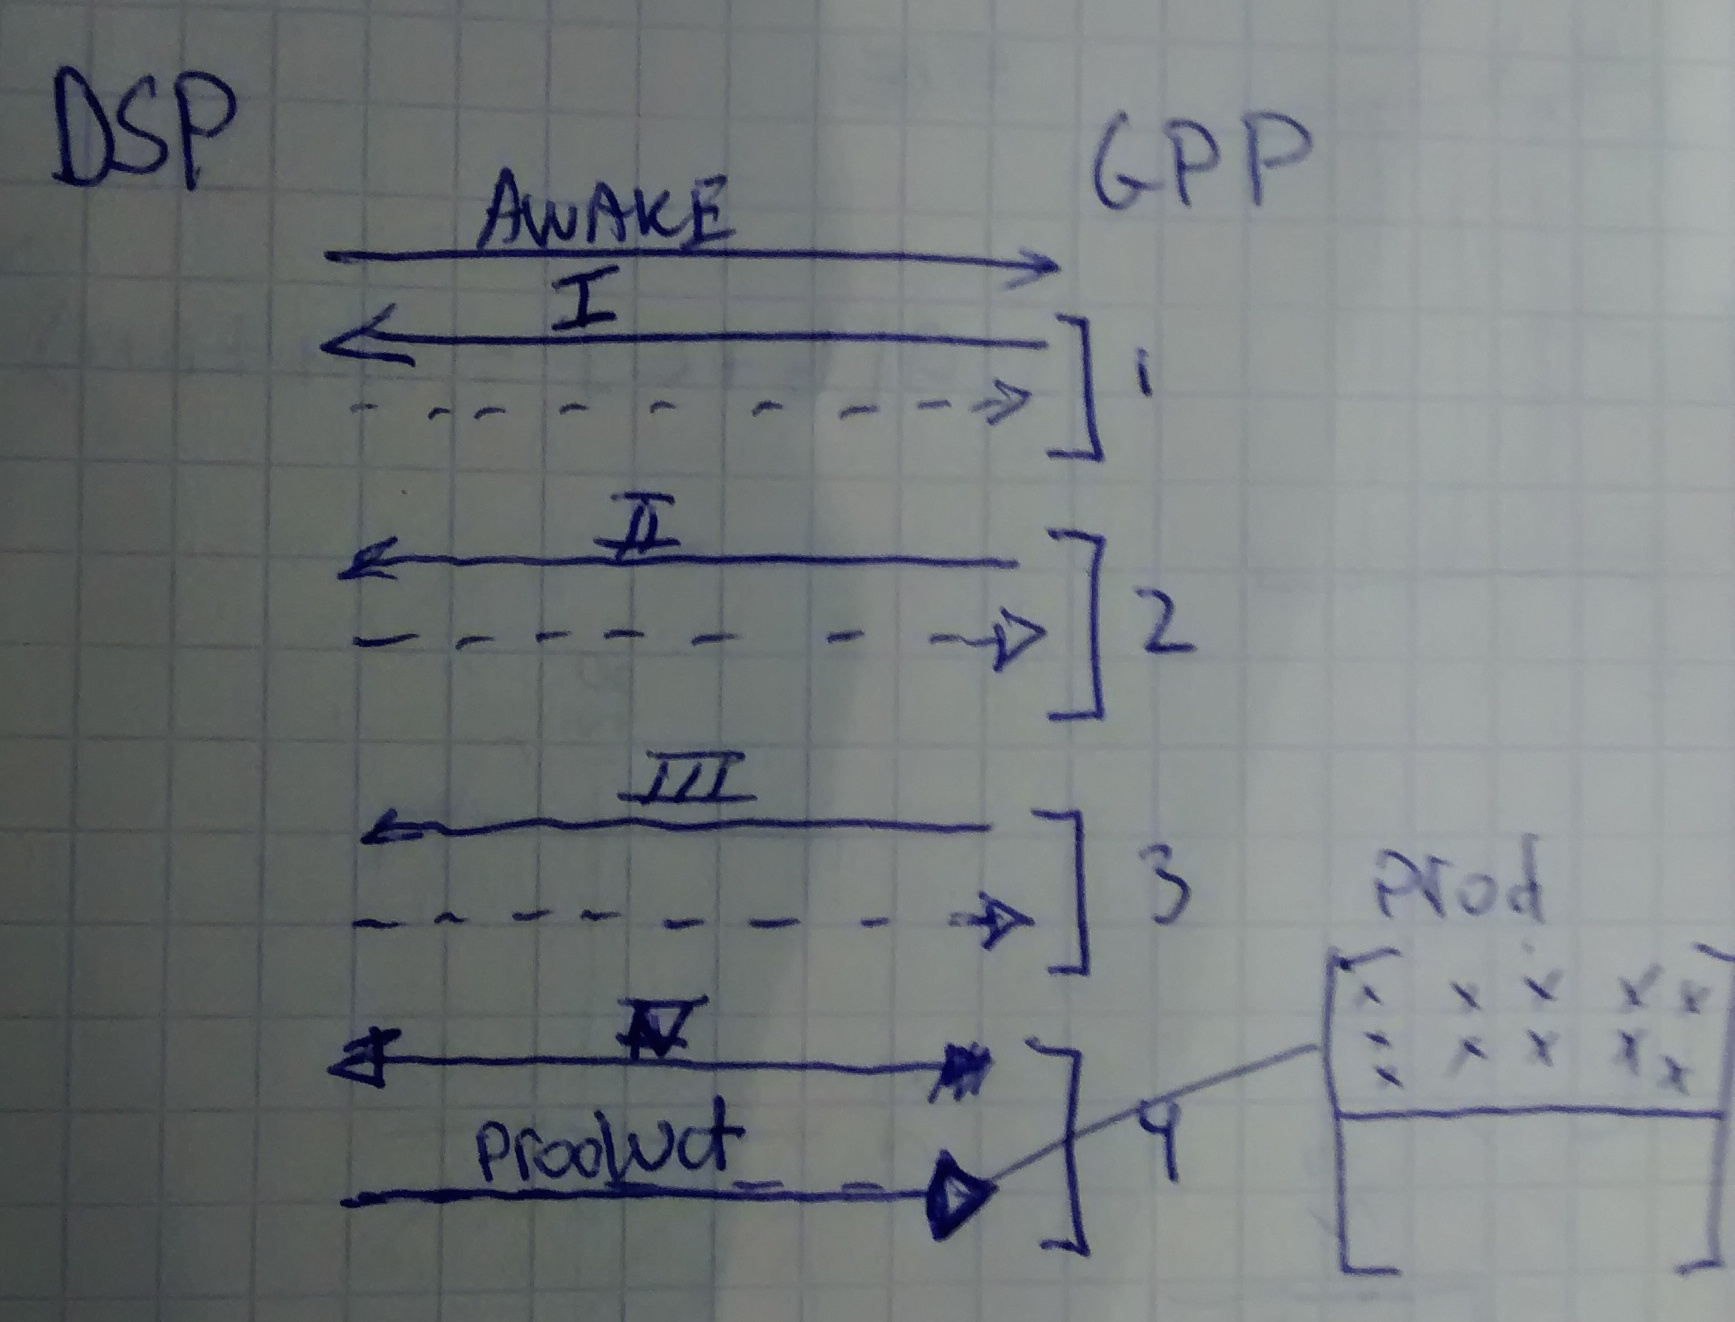
\includegraphics[width=\textwidth]{images/gpp_dsp_com}
\caption{Describing the communication process between the cores over time}
\label{fig:gpp_dsp_com}
\end{figure}

Unfortunately the communication API is slightly verbose and hard to handle.
For example, the sender has to allocate memory for a message, send it and the
receiver has the possibility to send it back, or free the message. If we opted
for the latter and re-allocate every message we would always crash the DSP core.
The former option would mean that if we wanted to send more than one message
directly from the GPP, the DSP would have to send the entire message back first.
We however observed that the communication overhead is negligible, so we
decided to always re-use the same message. The general communication time-line
is described in figure~\ref{fig:gpp_dsp_com}. One observation in this time-line
is that we send data six times. The reason why will be discussed in the next
section.

\subsubsection{Message Format}
We used the existing reference communication implementation and it's message
structure, but we extended it with our own matrices and an extra field that
indicates how big the resulting matrix should be. One thing we had to do 
was determine the maximum matrix size we could assign, such that it would fit 
in one message. This message would be stored inside a section of
\emph{APP\_BUFFER\_SIZE} large, thus our message structure has to fit in there. 
We experimentally found that we could send up to around 90k bytes per message.

The source matrices are 16 bit, but the result should be at least 32 bits. 
To accommodate for both 
situations in the same control message structure while optimally using our
message in a uniform way, we opted to use a \emph{union} structure so we 
can either send two 16 bit matrices or one 32 bit matrix at a time. The 
structure is given in figure~\ref{code:control_msg}. 

Because we have to send up to $128*128*2*2=65.536$ (2 matrices of 16 bits)
bytes from the GPP to the DSP, we need at least four messages considering
our bandwidth limit of 90k bytes. Thus we send the source in four messages, 
each containing a quarter of both matrices. The DSP only calculates a half of
the result matrix, making two messages sufficient: this results in six 
communication steps.

\begin{figure}[h]
\begin{lstlisting}[language=C]
struct mat2x16 {
	int16_t mat1[SIZE][SIZE];
	int16_t mat2[SIZE][SIZE];
};

struct mat32 {
	int32_t mat1[SIZE][SIZE];
};

typedef union {
	struct mat2x16 m16;
	struct mat32 m32;
} mat_t;

#define ARG_SIZE 256
typedef struct ControlMsg
{
    MSGQ_MsgHeader header;	// 20 bytes
    Uint16 command;				// 2 bytes
    Char arg1[ARG_SIZE];		// 256 bytes
    Uint8 size;					// 1 byte
    mat_t mat;						// 4 * SIZE * SIZE bytes
} ControlMsg;
\end{lstlisting}
\caption{The message structure we used}
\label{code:control_msg}
\end{figure}

\section{NEON}
To improve the performance of media and signal processing, 
\emph{NEON} SIMD technology is implemented in the \emph{Cortex-A8} core of the \emph{OMAP 3530} GPP. 
\emph{NEON} SIMD technology, which is also known as Advanced SIMD extension, 
takes the advantage of parallel operation to achieve the speed up.
\subsection{SIMD}
To understand NEON technology, the idea of SIMD is introduced at first. 
SIMD (Single Instruction Multiple Data) describes a way to perform the same operation on multiple data with same type and size in a single instruction. 
The idea of parallel operation comes from the fact that most of multimedia data are 16-bit or 8-bit wide, while the general purpose registers are 32-bit wide. 
To effectively utilize the space of registers, simultaneous computation is developed.  
\subsection{NEON Technology} 
\emph{NEON} technology, as the Advanced SIMD extension in \emph{Cortex-A8}, performs SIMD operations in group. 
NEON instructions operate on vectors stored in 64-bit or 128-bit registers, 
then vectors of elements with same type can perform the same operation on multiple items at the same time.
Figure~\ref{fig:neon} shows how multiple items are computed simultaneously. 

\begin{figure}[h]
\centering
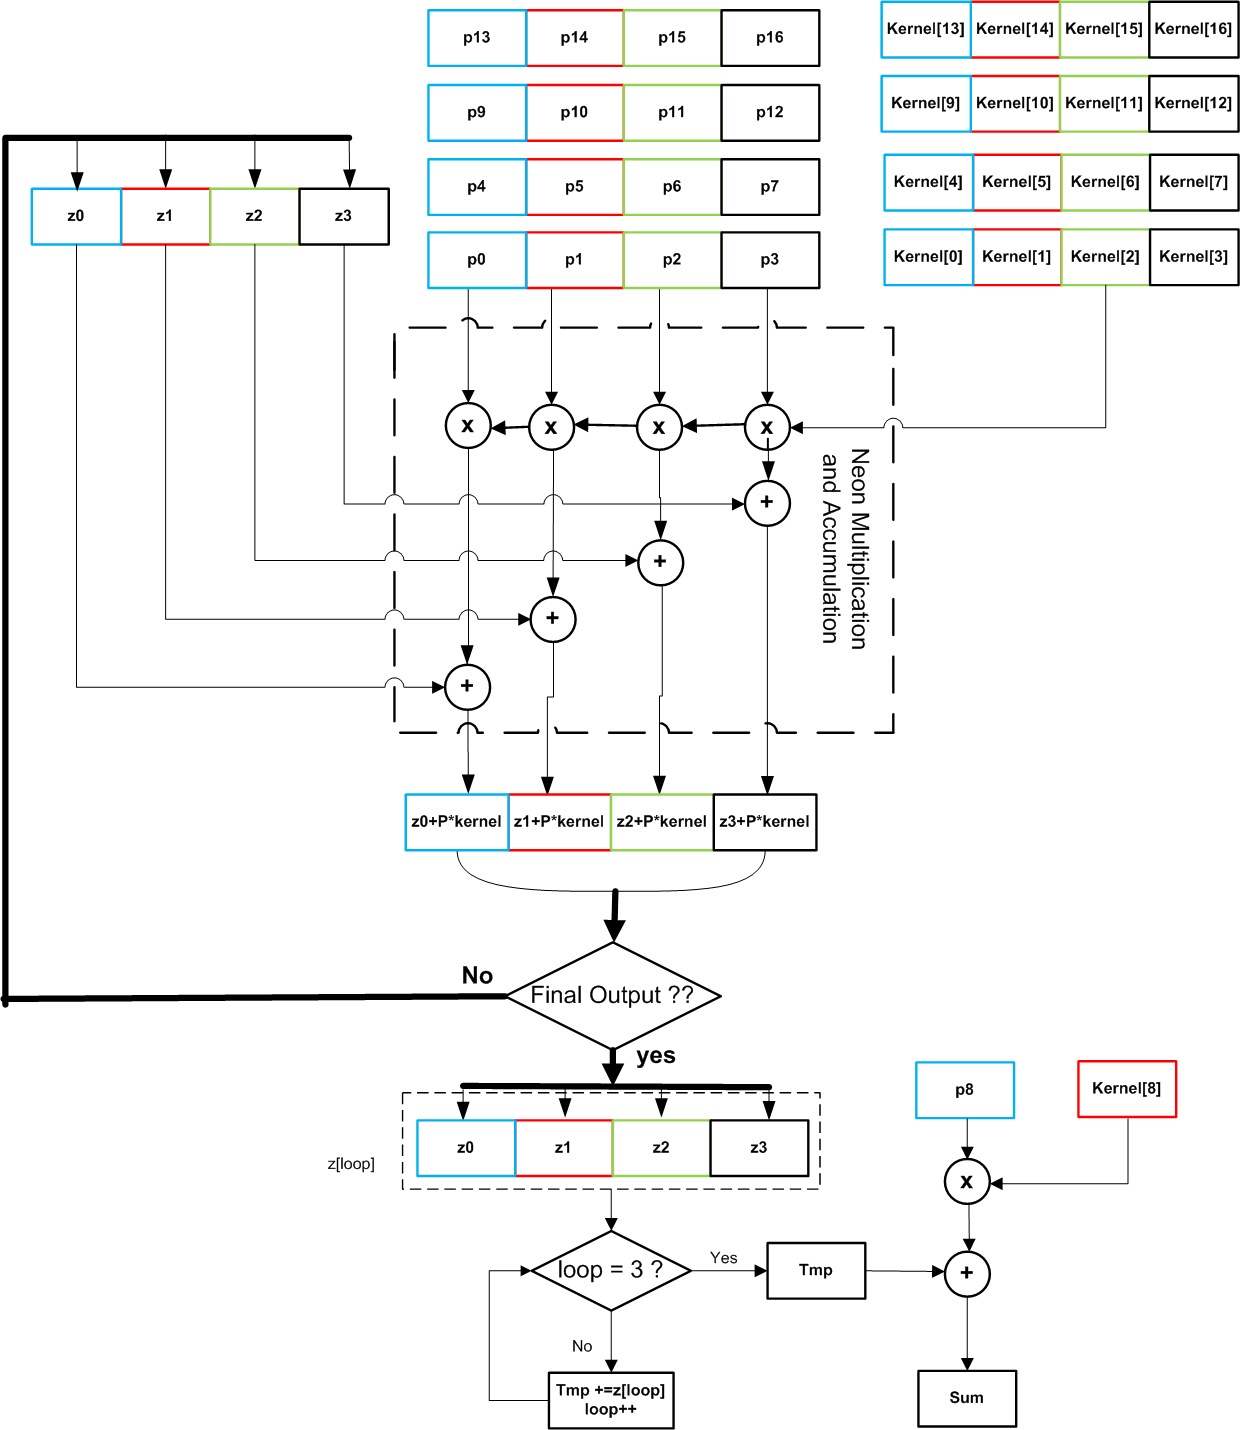
\includegraphics[width=0.9\textwidth]{images/neon}
\caption{Parallel computing based on NEON}
\label{fig:neon}
\end{figure}

\subsection{Hardware Features}
The NEON architecture has the following features\cite{hardware}:
\begin{enumerate}
\item \emph{16-Entry instruction queue}
\item \emph{32 x 64-bit general purpose registers in register file.}
These registers can alternatively be viewed as 16 x 128-bit registers
\item \emph{6-stage execution pipeline.}
NEON supports either integer or single precision floating point execute pipeline.
\item \emph{Load/store and permute pipeline}
\item \emph{12-Entry load data queue}
\end{enumerate}

\subsection{Implementation}
To enable the built-in intrinsics of NEON, 
\emph{$-$mfpu$=$neon}\cite{ARMoptions} is used during compiling time.
Also, the header file \emph{arm\_neon.h} is included 
to support NEON intrinsics in the c file.
In our case, the incoming message contains the matrix with data of 16-bit wide, 
and then after calculation, when the final outcome is sending back to GPP, the data size is 32-bit to avoid overflow.
In the following section, NEON intrinsics that are used for parallel computing in our experiment are explained.

\subsubsection{Vector Data Type}
Neon defined its own data type\cite{DataType} for multiple data operation, the format is given as:
~\\ 
\textbf{ \textless type\textgreater \textless size\textgreater x\textless number of lanes\textgreater\_t}

For example, the data type we are going to use in NEON is \emph{uint32x4\_t}, 
which means the vector has four lanes, 
with each of the them containing an unsigned 32-bit integer. 

\subsubsection{NEON Intrinsics}
NEON intrinsics \cite{Intrinsics} provide groups of functions for operation. 
In our case, functions related to load, multiplication and addition are used. 
\begin{enumerate}
\item \textbf{uint32x4\_t  vmovq\_n\_u32(uint32\_t value)}

This intrinsic loads all lanes of vector to the same input value. 
The input value is an unsigned 32-bit integer, 
while the four lanes being loaded each contains an unsigned 32-bit as well.


\item \textbf{int32x4\_t   vld1q\_s32(\_\_transfersize(4) int32\_t const * ptr)}

This intrinsic loads a single value from memory to all lanes.
The data stored in memory is signed 32-bit integer, 
while the four lanes each contains a signed 32-bit integer.

\item \textbf{int32x4\_t   vmlaq\_s32(int32x4\_t a, int32x4\_t b, int32x4\_t c)}

This intrinsic multiplies b by c, and accumulates the result with a in all four lanes.
The final results are then stored in four lanes as well.
\end{enumerate}

\subsubsection{Multiplication Algorithm}

In order to fully utilize the Neon resources, we have used following algorithm to compute the matrix multiplication. The following illustration shows one rows of results.
The input matrices are following:

$$
\begin{pmatrix}
 x1 	& \color{red}{x2} 	& \color{green}{x3} & \color{blue}{x4}\\
 x5 	& x6 				& x7&x8\\
 x9 	& x10 				& x11&x12\\
 x13 	& x14 				& x15&x16\\
\end{pmatrix}
\times
\begin{pmatrix}
y1&y2&y3&y4\\
y5&y6&y7&y8\\
y9&y10&y11&y12\\
y13&y14&y15&y16\\
\end{pmatrix}
$$


The output matrix would be : 
=
\begin{table}[h]
	\resizebox{\textwidth}{!}{
		$\left(
			\begin{tabular}{cccc}
				x1y1+\color{red}{x2}y5\color{black}{+}\color{green}{x3}y9\color{black}{+}\color{blue}{x4}y13&x1y2\color{black}{+}\color{red}{x2}y6\color{black}{+}\color{green}{x3}y10\color{black}{+}\color{blue}{x4}y14&x1y3\color{black}{+}\color{red}{x2}y7\color{black}{+}\color{green}{x3}y11\color{black}{+}\color{blue}{x4}y15&x1y4\color{black}{+}\color{red}{x2}y8\color{black}{+}\color{green}{x3}y12\color{black}{+}\color{blue}{x4}y16\\
				-&-&-&-\\-&-&-&-\\-&-&-&-\\
			\end{tabular}
		\right)$
	}
\end{table}

In the output matrix, the elements with the same color are multiplied by the Neon at the same time. In this way, Neon produces the results of 4 multiplications at the same time. In the output row above, x1y1, x1y2, x1y3 and x1y4 are produced by the neon simultaneously. However, these are just the partial results for the first row of output matrix. In order to get the complete results for the first row these partial results should be added to the other partial results of the same row. This complete task of multiplication and addition is done by using \emph{Multiplication and Addition} functional unit of neon. The conceptual diagram of this multiplication and addition is shown in figure~\ref{fig:neon_mult_add}.

\begin{figure}[h]
\centering 
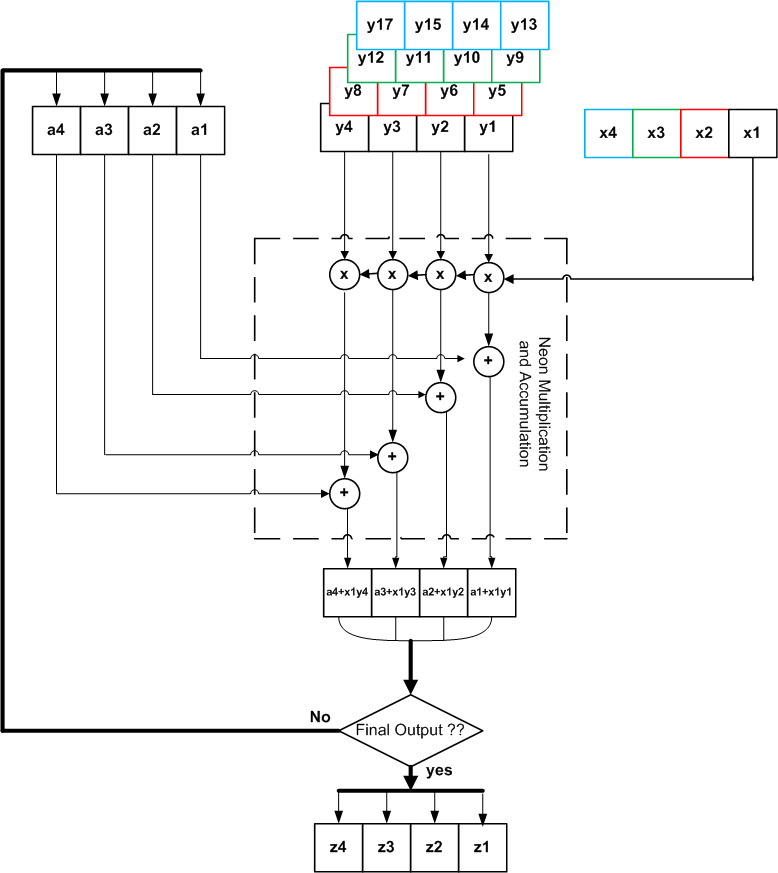
\includegraphics[width= 0.7\textwidth]{images/MandA}
\caption{Parallel Multiplication and Addition with Neon  }
\label{fig:neon_mult_add}
\end{figure}

\subsection{Optimization flags}

The following compiler flags are used to perform optimization during the compilation of source code:

\begin{itemize}
\item{\textit{O3:}} provides the highest level of optimization of code for the execution time and code size
\item{\textit{mtune=cortex-a8:}} tunes the generated code to run faster on \emph{cortex-a8} than any other processor of same architecture
\item{\textit{march=armv7-a:}} takes the CPU name \emph{armv7-a} and allows the gcc to generate a code that uses all the features of that family
\item{\textit{mfloat-abi=softfp:}} specifies which floating point \emph{Application Binary Interface} (ABI)to use. By specifying \emph{mfloat-abi=softfp}, \emph{gcc} is allowed to generate code by using the hardware floating point units, but still using the \emph{soft-float} calling convention
\item{\textit{mfpu=neon:}} specifies what floating-point hardware (or hardware emulation) is available on the target
\end{itemize}

Moreover, the following flags were used: \emph{ftree-vectorize}, \emph{ffast-math} and \emph{fomit-frame-pointer} Nevertheless, no additional benefit in terms of speedup was observed because they are implicitly enabled if the \emph{-O3} optimization flag is used.




\input{Analysis}

\section{Conclusion}
\label{sec:Conclusion}
 In this report we have described the optimization process of a sequential image processing algorithm on a heterogeneous system with multiple processing units.
By profiling the reference application we were able to focus our attention on the most compute intensive function of the reference application.
At first we simply implemented that function on each available processing core independently and performed timing measurements. By applying minor changes to the code, the two cores were merged together to work in parallel.
By timing each of the calculations independently, the workload among the two available processing units were properly balanced.
This lead to the minimization the idle time of a processor that waits for the other one for synchronization purpose to continue execution.
Throughout the development many optimization techniques were experimented with such as compiler flags, manual loop unrolling etc.
Eventually a speedup of a factor of two and above was achieved. Due to the nature of optimizations some errors were introduced in the results. Nevertheless after extensive error analysis it was concluded that the errors are negligible and hence acceptable. Several other methods and techniques could be used to further increase the speedup which are mentioned in the future work section.

\section{Future Work}
\label{sec:Future Work}
Several changes could be made to the current application that could possibly improve the results even more.
First of all, further optimization are possible within the DSP and the NEON block. 
For instance in NEON, floating point calculations are used at the moment. But more speedup can be achieved by using fixed-point calculations because in general fixed-point calculations are faster than floating-point calculations.
Secondly, other functions could possibly be computed in parallel as well.
i.e. The \textit{non\_max\_supp() \& apply\_hysteresis()} are the next computationally intensive applications taking 8\% and 5\% each respectively.
Even more, simply utilizing NEON in those functions could potentially speed up the overall implementation.

\section{Appendix}
\begin{figure*}[h!]
    \centering
    \begin{subfigure}[b]{0.3\textwidth}
            
\includegraphics[width=\textwidth]{square_baseline}
            \caption{The baseline result}
            \label{fig:app_square_baseline}
    \end{subfigure}
    \begin{subfigure}[b]{0.3\textwidth}
            
\includegraphics[width=\textwidth]{square_out}
            \caption{The optimized result}
            \label{fig:app_square_out}
    \end{subfigure}
    \begin{subfigure}[b]{0.3\textwidth}
            
\includegraphics[width=\textwidth]{square}
            \caption{The original picture}
            \label{fig:app_square}
    \end{subfigure}

    \begin{subfigure}[b]{0.3\textwidth}
            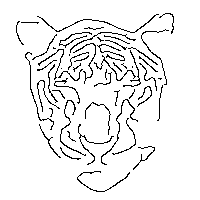
\includegraphics[width=\textwidth]{tiger_baseline}
            \caption{The baseline result}
            \label{fig:app_tiger_baseline}
    \end{subfigure}
    \begin{subfigure}[b]{0.3\textwidth}
            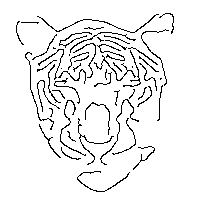
\includegraphics[width=\textwidth]{tiger_out}
            \caption{The optimized result}
            \label{fig:app_tiger_out}
    \end{subfigure}
    \begin{subfigure}[b]{0.3\textwidth}
            
\includegraphics[width=\textwidth]{tiger}
            \caption{The original picture}
            \label{fig:app_tiger}
    \end{subfigure}

    \begin{subfigure}[b]{0.3\textwidth}
            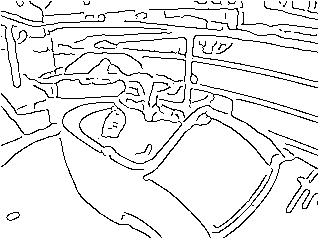
\includegraphics[width=\textwidth]{klomp_baseline}
            \caption{The baseline result}
            \label{fig:app_klomp_baseline}
    \end{subfigure}
    \begin{subfigure}[b]{0.3\textwidth}
            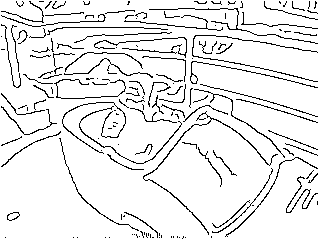
\includegraphics[width=\textwidth]{klomp_out}
            \caption{The optimized result}
            \label{fig:app_klomp_out}
    \end{subfigure}
    \begin{subfigure}[b]{0.3\textwidth}
            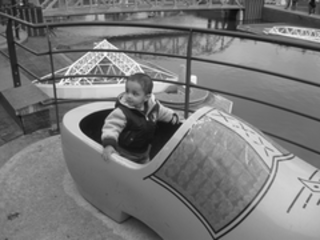
\includegraphics[width=\textwidth]{klomp}
            \caption{The original picture}
            \label{fig:app_klomp}
    \end{subfigure}
    \caption{The three different images used to test the implementation}
    \label{fig:imgdiff}
\end{figure*}


\bibliography{references}{}
\bibliographystyle{unsrt}

\end{document}
